% Template for PLoS
% Version 1.0 January 2009
%
% To compile to pdf, run:
% latex plos.template
% bibtex plos.template
% latex plos.template
% latex plos.template
% dvipdf plos.template

\documentclass[10pt]{article}

% amsmath package, useful for mathematical formulas
\usepackage{amsmath}
% amssymb package, useful for mathematical symbols
\usepackage{amssymb}

% graphicx package, useful for including eps and pdf graphics
% include graphics with the command \includegraphics
\usepackage{graphicx}

% cite package, to clean up citations in the main text. Do not remove.
\usepackage{cite}

\usepackage{color} 

% Use doublespacing - comment out for single spacing
%\usepackage{setspace} 
%\doublespacing


% Text layout
\topmargin 0.0cm
\oddsidemargin 0.5cm
\evensidemargin 0.5cm
\textwidth 16cm 
\textheight 21cm

% Bold the 'Figure #' in the caption and separate it with a period
% Captions will be left justified
\usepackage[labelfont=bf,labelsep=period,justification=raggedright]{caption}

% Use the PLoS provided bibtex style
\bibliographystyle{plos2009}

% Remove brackets from numbering in List of References
\makeatletter
\renewcommand{\@biblabel}[1]{\quad#1.}
\makeatother


% Leave date blank
\date{}

\pagestyle{myheadings}
%% ** EDIT HERE **


%% ** EDIT HERE **
%% PLEASE INCLUDE ALL MACROS BELOW

%% END MACROS SECTION

\begin{document}

% Title must be 150 characters or less
\begin{flushleft}
{\Large
\textbf{How to Eliminate the Unnecessary So That The Necessary May Speak. Biological Reference Points.}
}
% Insert Author names, affiliations and corresponding author email.
\\
Laurence T. Kell$^{1,\ast}$, 
Paul De Bruyn$^{2}$, 
Finlay Scott$^{3}$
Richard D.M. Nash$^{4}$
\\
\bf{1}  ICCAT Secretariat, C/Coraz\'{o}n de Mar\'{\i}a, 8. 28002 Madrid, Spain.
\\
\bf{2}  AZTI Tecnalia. Herrera kaia portualdea z/g, 20110 Pasaia, Gipuzkoa, Spain
\\
\bf{3}  The Fisheries Laboratory, Lowestoft, NR33 0HT, Suffolk, England
\\
\bf{4}  Institute of Marine Research, PO Box 1870 Nordnes, 5817 Bergen, Norway
\\
$\ast$ E-mail: Corresponding Laurie.Kell@iccat.int
\end{flushleft}

% Please keep the abstract between 250 and 300 words
\section*{Abstract}

% Please keep the Author Summary between 150 and 200 words
% Use first person. PLoS ONE authors please skip this step. 
% Author Summary not valid for PLoS ONE submissions.   
\section*{Author Summary}

\section*{Introduction}

%The ability to simplify means to eliminate the unnecessary so that the necessary may speak.  ~Hans Hofmann, Introduction to the Bootstrap, 1993

The adoption of the Precautionary Approach to fisheries management \cite{garcia1996precautionary}  requires a formal consideration of uncertainty. An important principle 
of the approach is that the level of precaution  should increase as uncertainty increases, e.g. from data rich to poor situations. However, defining stocks
as data rich or data poor based purely on the availability of catch and effort data obscures the fact that considerable uncertainty often exists about the 
biological processes such as natural mortality, recruitment processes and stock structure of commercially important fish stocks. Conversely even when data are limited, empirical studies have shown that life history parameters, 
such as age at first reproduction, natural mortality, and growth rate are strongly correlated. Therefore biological knoweledge is important both
for evaluating the robustness of advice obtained from data-rich stock assessments and in allowing general rules, for example about choice of reference points (indicators of the status of a stock e.g. biomass too low or fishing pressure too high etc), 
to be derived for all stocks.

Fisheries management is concerned with trying to set, and then achieve, realistic managment objectives. This is carried out through defining
management measures of interest, for example spawning stock biomass (SSB) and fishing mortality (F), and then
setting values of a range of reference points for these measures. These reference points can be used as targets, for example $B_{MSY}$, or limits, for example, $F_{crash}$.
However, achieving these management objectives is made difficult by, amongst other things, the impact of
biological and ecological uncertainty on the dynamics of the stock.
% Chuck in some suitable references here
A key question for fisheries management is therefore how can research be prioritised so that the impact of biological uncertainty on achieving management
objectives can be reduced?
Answering this question requires the estimation of the relative importance of the underlying biological assumptions made about the stock with respect to
the managment measures of interest.  
For example, does uncertainty about the stock recruitment relationship have a relatively bigger effect on yield and sustainability than uncertainty about natural mortality?

Senstivity and elasticity analyses can be used to evaluate the effect of changes in system parameter values on system outputs. They are commonly used in
financial and economic managment, but have also have been applied to biology and conservation~\cite{de1986elasticity}.
Such analyses can be used within fisheries management to identify the stock assumptions that have the greatest impact on management measures
and therefore where the impact of uncertainty may have the greatest effect on achieving managment objectives.
Sensitivities measure absolute changes, for example, by how much does the estimate of MSY change as the value of length of first maturity changes.
While elasticities measure the relative change and can be used to compare between a range of different sources of uncertainty. For example, 
does the length of first maturity have a larger proportional impact on estimates of MSY than the steepness of the stock recruitment relationship?
Elasticity analysis has  proven to be a useful tool in a number of areas of population and conservation biology, for example relating changes in
vital rates to changes in the population life history~\cite{grant2003density} and to quantities of importance in management such as population
viability~\cite{heppell1998application}. Previously, elasticity anaysis has focused on terrestrial 
ecology ~\cite{Benton1999467, Hunter2000299, Pichancourt200631} with limited application to marine populations ~\cite{RogersBennett2006, Heppell2007}. 
The applicability of this approach to resource management has therefore been demonstrated and here use it to evaluate the relative importance of
the biological assumptions made in fishery stock assessment. that are too seldom questioned.


A fuller consideration of uncertainty within fisheries advice frameworks can be performed used Bayesian approaches or Managemement Strategy Evaluation (MSE).
MSE is commonly used to evaluate the impact of different managment measures, given a broad range of uncertainty. However,
performing an MSE is a costly process in terms of human resources and can take several years. Therefore, tools such as elasticity analysis, which
is comparatively less demanding to carry out, are important to 
help identify and focus research and management efforts. For example, is it more important to reduce uncertainty about the stock 
recruitment relationship or natural mortality or to develop harvest control rules that are robust to such uncertainty? Elasticity analyses can 
be used to answer such questions and prioritise research effort. It can also shift the current focus from defining stocks either as data poor or rich 
defined solely on fishery catch and effort towards a better understanding of biological processes. 

Here we demonstrate the use of elasticity analysis for prioritising research effort with a study of the population dynamics of a fish stock based on life history theory. As such the study is not modelled on one specific species of fish.
We do this by first simulating a stock based on life history relationships~\cite{gislason2008coexistence} 
and then by projecting the stock from an unfished to 
an over-exploited state. We do this in order to compute elasticites to allow us to evaluate the relative importance of the different system or biological parameters
when assessing the stock relative to system characteristics defined by biological reference points. This allows us to address two important questions i.e. what is
the relative importance of the different biological processes in providing advice and and how robust is advice based on the common biological reference 
points.


% You may title this section "Methods" or "Models". 
% "Models" is not a valid title for PLoS ONE authors. However, PLoS ONE
% authors may use "Analysis" 
\section*{Materials and Methods}

Empirical studies have shown that in teleosts there is significant correlation between the life history parameters  
such as age at first reproduction, natural mortality, and growth rate \cite{roff1984evolution}. Additionally, size-spectrum theory 
and multispecies models suggest that natural mortality scales with body size \cite{andersen2006asymptotic}, 
\cite{pope2006modelling} \cite{gislason2008coexistence}. This means that from something that is easily observable, like the maximum size,
it is possible to infer the life history parameters of species for which data are not easily observable or available.

\cite{gislason2008coexistence} summarised life history characteristics and the relationships between them for a range of stocks and species. 
These relationships were used to parameterise an age-structured population model using relationships that describe growth, maturation and natural mortality.
This population was then projected at a constant fishing mortality until equilibrium was reached for a wide range of fishing mortalities.

The analysis allows us to evaluate where more biological knowledge is needed and to identify robust reference points for use in management. Following this analysis
sensitivy analysis could be conducted to help quantify the costs and benefits and MSE to develop robust management advice.

SSB and fishing mortality ($F$) relative to the corresponding quantity estimated from each of the $F_{MSY}$, $F_{0.1}$ and $F_{Crash}$ reference points were used 
as indices of stock status and exploitation. In the case of a fishing mortality equal to $F_{Crash}$, SSB is 0, by definition, therefore an SSB corresponding to
75\% of $F_{Crash}$ was used.  $F_{MSY}$ corresponds to the level of exploitation that provides the maximum 
sustainable yield,  $F_{0.1}$ is a proxy for $F_{MSY}$ and is the fishing mortality that corresponds to a point on the yield per recruit curve where the slope is 
10\% of that at the origin) and  $F_{Crash}$ the level of F that will drive the stock to extinction. 

The elasticities of these indices in each year relative to the parameters in model were then used to
evaluate the relative importance of the various processes (i.e. growth, maturation, stock recruitment, natural mortality and selectivity of the fishery)
and the parameterisation of those process (e.g. $K$ the rate of growth and $L_{\infty}$) with respect to stock status. 

The calculation of reference points and fishing mortality also  depend upon the selection pattern,  
since not all ages are equally vulnerable to a fishery. If there is a refuge for older fish, a higher level of fishing effort will be sustainable.
Also, if the fecundity of older fish is greater than the fecudity of younger fish of the same mass-at-age, e.g. due to maternal effects or repeat
spawners being more fecund then a condideration of the interactions between biology and selectivity will be important.

\subsection{Life History Relationships}

The Russell equation \cite{russell1931some} summarises the key processes influencing the dynamics of exploited populations i.e.
 
\begin{equation}f(B_2) = B_1 + (G + R) - (F+M)\end{equation}

where a biomass $B_2$ is a function of the biomass in the year before ($B_2$,gains due to growth (G) and recruitment (R) and  losses due to fishing (F) and natural 
mortality (M). Two other factors which have also been recognised since Russel originally formulated this equation are the gains through immigration (I) and losses through emigration (E)thus modifying the original equation to:

\begin{equation}f(B_2) = B_1 + (G+R+I) - (F+M+E)\end{equation}

The knowledge about these processes affects our ability to provide robust scientific advice. In this paper we concentrate 
on G,R,F and M as we assume a single heterogenerous population with out emmigration or immigration; However our approach could be extended to include I and E.

Life history relationships were used to parameterise appropriate functional forms for the various processes in order to provide a generic framework for
modelling stock dymanics. This allows processes to be modelled under a variety of assumptions, for a range of species and for the impact of the various parameters
to be evaluated.  


\begin{description}
    \item[Growth] is modelled by the Von Bertalanffy growth equation \cite{von1957quantitative}

      \begin{equation} L_t = L_{\infty}(1 - L_{\infty}exp(-k(t-t_0)) \end{equation}
         
where $K$ is the rate at which the rate of growth in length declines as length approaches the asymptotic length  $L_{\infty}$ 
and $t_{0}$ is the time at which an individual is of zero length. 

Length is converted to mass using the condition factor, $a$ and allometric growth coefficient, $b$.

\begin{equation} W = a \times L_t^b \end{equation}

 \item[Recruitment] is split into Stock Reproductive Potential (SRP) and the stock recruitment relationship (SRR).

SRP is the sum of the products of the numbers of females, $n$, proportion mature-at-age, $Q$ and their mean fecundity-at-age, $F$, i.e. 

   \begin{equation} SRP = \sum{n \times Q \times F } \end{equation}

where their mean fecundity-at-age is equal to 
\begin{equation} F = a \times L^{b\prime} \end{equation}

if $a$ and $b$ are the same as in equation 3 then SRP is equivalent to female spawning stock biomss (SSB). However, generally the fecundity to length relationship differs from the weight to length relationship due to variations caused by fish condition and age effects altering the relationship between weight and eggs produced (P�rez-Rodr�guez et al. 2011).

Proportion mature is modelled by the logistic equation with 3 parameters: age at 50\% mature, age at 95\% mature and the asymptotic value $asym$. The 
latter allows SRP to not be equivalent to stock mass-at-age.

\begin{equation}
f(x) = \left\{ \begin{array}{ll}
			0                                 &\mbox{ if $(a50-x)/ato95 >  5$} \\
			asym                              &\mbox{ if $(a50-x)/ato95 < -5$} \\
			\frac{asym}{1.0+19.0^{(a50-x)/ato95)}} &\mbox{ otherwise}
		\end{array}
       \right.
\end{equation}

%Parameters can be derived as in \cite{williams2003implications} from the theoretical relationship between $M$, $K$, and age at maturity $a_{Q}$ based on the dimensionless ratio of length at maturity to asymptotic length \cite{beverton1992patterns}.
Here the value of $a50$ comes from the empirical relationship between $L_{\infty}$ and age at maturity \cite{gislason2008coexistence}:

\begin{equation}
  a50=0.72 logL_{\infty}^{0.93}
\end{equation}

We use a Beverton and Holt stock recruitment relationship reformulated in terms of steepness ($h$), virgin biomass ($v$) and $S/R_{F=0}$, 
where steepness is the ratio of recruitment at 20\% of virgin biomass to virgin recruitment ($R_0$). 

For the BevertonHolt stock-recruit formulation:

\begin{equation}
R=\frac{0.8 \times R_0 \times h \times S}{0.2 \times S/R_{F=0} \times R_0(1-h)+(h-0.2)S}
\end{equation} 

Steepness is difficult to estimate from stock assessment data sets and there is often insufficient range in biomass levels that is required for its estimation \cite{ISSF2011steep}.
Steepness and virgin biomass were set to 0.9 and 1000 t respectively.

\item[Natural mortality]
at size is derived from the life history relationship \cite{gislason2010does}.
               
\begin{equation}
            M = exp(M1 + M2 log(L) + 1.51log(L_{\infty}) + 0.97log(k) + a[5]/T),
\end{equation} 
where $M1$ (which determines the average natural mortality) = -2.11, $M2$ (which determines the rate at which natural mortality declines with length) = -1.70 and $L$ is the average length of the fish (in cm) for which the $M$ estimate applies. Here we use the length at mid-year
to calculate the natural mortality at age.


\item[Selection pattern] 
of the fishery can be represented by a double normal 
(see \cite{Hilbornetal2000}) with three parameters that describe the age at maximum selection ($a1$), the rate at which the lefthand 
limb increases ($sl$) and the righthand limb decreases ($sr$) which allows flat topped or domed shaped selection patterns to be chosen.

Even in data poor situtations where catch-at-age for the entire catch time series is not available, some data will normally exist for 
some years or gears or for similar stocks and species. In cases where some length frequency data are available the shape of selection pattern, i.e.
age at recruitment to the fishery, can be estimated using a method like that of \cite{wetherall1987estimating}. This allows
a double normal curve to be parameterised, i.e. age at maximum selectivity and whether the selection pattern is flat topped or dome shaped.

\begin{equation}
f(x) = \left\{ \begin{array}{rl}
 2^{-[(x-a_1)/s_L]^2} &\mbox{ if $x<a_1$} \\
 2^{-[(x-a_1)/s_R]^2} &\mbox{ otherwise}
       \end{array} \right.
\end{equation}
 
\end{description}

\subsection{Seasonality}

The model is a discrete population model where the number of individuals in a year-class in a year is a function of the number of individuals in the previous year.
However, processes like growth, maturation, natural mortality and fishing occur in different seasons of the year. Therefore to take account of this the age for which
the expected values of mass, maturity and natural mortality-at-age can vary.
For the stock mass and lengths-at-age are calculated at spawning time, catch mass-at-age is calculated in mid year and natural mortality is a function of the lengths-at-age 
mid year.  

\subsection{Stock projections}
Using the relationships described above we generate a fully specified age-structured stock based on a value of $L_{\infty}$=100 cm. The stock is projected
forward through time at different levels of constant fishing pressure ranging from no fishing ($F$=0) to over exploited ($F=F_{crash}$).
The management measures of interest are the equilibrum SSB, yield and biomass relative to their reference point values corresponding to
$F_{MSY}$, $F_{0.1}$ (a proxy for $F_{MSY}$) and $F_{crash}$, a limit reference point, e.g. $SSB / SSB_{MSY}$, $SSB / SSB_{F0.1}$ etc.

$F_{0.1}$ is the fishing mortality on the yield per recruit curve where the slope is 10\%  of that at the origin, a conservative proxy for $F_{MSY}$.
$F_{Crash}$ is the fishing mortality that will drive the stock to extinction since it is equivalent to a R/S greater than the slope at the origin of
the stock recruitment relationship, i.e. recruitment can not replace removals for a fishing mortality equal to $F_{Crash}$.  

\subsection{Elasticity}
As mentioned above, elasticity analysis can be used to measure the proportional change of a system characterisic to a change in a system parameter. 
The general equation for calculating the elasticity of system characteristic $y$ with respect to system parameter $x$ is:

\begin{equation}
E_{y,x} = \left| \frac{\partial \ln y}{\partial \ln x} \right|        
%%     = \left| \frac{\partial  y}{\partial  x} \cdot \frac{x}{y} \right|
%%       \approx \left| \frac{ \%\bigtriangleup  y}{\%\bigtriangleup x} \right|  
%
\end{equation} 

The absolute value operator is used for simplicity although the elasticity can also be defined without the absolute value operator when the direction of 
change is important, e.g. to evaluate if a reduction in natural mortality increases or decreases MSY reference points.	

Here we calculate the elasticities of the management measures described above with respect to the life history and selectivty parameters grouped into the
categories: growth ($K$, $t_0$, $a$, $b$, $L_{\infty}$), maturity ($a50$, $ato95$ and $asym$), natural mortality ($M1$ and $M2$), the stock recruitment
relationship ($h$ and $vb$) and the selectivity ($a1$, $sl$ and $sr$). For example, the elasticity of $SSB$ relative to $SSB_{MSY}$ with respect to $L_{\infty}$ is calculated as:

\begin{equation}
E_{SSB_{MSY},L_{\infty}} = \left| \frac{\partial \ln SSB_{MSY}}{\partial \ln L_{\infty}} \right|
\end{equation}

The elasticities are calculated for every level of $F$ used in the projections and therefore show how the current state of the stock and exploitation rate
affect the relative importance of the different life history parameters, i.e. where the most important source of uncertainty is.

Note that although the parameter values for $K$, maturity and natural mortality at age are calculated using the value of $L_{\infty}$, these values are set
before the elasticities are calculated, i.e. the elasticities with respect to $L_{\infty}$ do not reflect the impact of $L_{\infty}$ on these life history
relationships, only on the impact of the stock dynamics through the von Bertalanffy growth equation.

% Results and Discussion can be combined.
\section*{Results}

The growth, natural mortality, proportion mature and selectivity-at-age of the stock are shown in Figure~\ref{fig:stock}.
The expected equilibrium dynamics, along with the MSY, $F_{0.1}$ and $F_{crash}$ reference points are shown in Figure~\ref{fig:brp}. 
The equilibrium dynamics over the range of fishing mortalities from 0 to $F_{crash}$ are presented as a phase plot (Figure~\ref{fig:kobe})
where the x-axis corresponds to $biomass$ relative to $B_{MSY}$ and the y-axis corresponds to $harvest$ relative to $F_{MSY}$.
Quadrants are defined for the 
stock amd fishing mortality relative to $B_{MSY}$ and $F_{MSY}$; i.e. red when $B<B_{MSY}$ and $F>F_{MSY}$, green if $B$ $\geq$ $B_{MSY}$ and $F$ $\leq$ $F_{MSY}$,
and yellow otherwise. I.e. the red quadrant refers to an overfished stock subject to overfishing, green to a stock which is neither overfished 
or subject to overfishing and the yellow to a stock which is either overfished stock or subject to overfishing.

Plots of the elasticities with respect to each life history parameter (grouped by life history process) for the range of fishing mortalities are presented in
Figures~\ref{fig:elasssb} and \ref{fig:elasf}.
The vertical line indicates the boundary between the red and green quadrants and the horizontal line where the value of the elasticity is 0,
i.e. where varying a parameter has no effect on the measure of interest.

The plots allows several important questions to be addressed, e.g. which processes and parameters have the biggest impact and whether certain reference points are more 
robust to uncertainty in key processes than others? Also does the importance of the life history parameter depend upon the stock status,
i.e. is knowledge on some parameters and processes more important when a stock is depleted than when it is within safe biological limits. Also
are F reference points for example more robust than those based on SSB.	

Inspection of the elasticities of relative SSB (Figure~\ref{fig:elasf}) [THIS SHOULD BE FIGURE 4] shows that the elasticities of SSB relative to $SSB_{MSY}$ and $SSB_{F0.1}$
are broadly similar.
For all three reference points the natural mortality parameters $M1$ and $M2$ have the biggest proportional effect on the relative SSB. 
The next most important parameter is $asym$ the selectivity parameter. 
The steepness of the stock recruitment relationship is important when considering SSB relative to $SSB_{MSY}$ and $SSB_{F0.1}$ but
less so relative to $SSB_{Fcrash}$.
The other processes (growth and maturity) have similar impacts to each other; the most important parameters are $K$,
age at 50\% mature and age at recruitment to the fishery.

When the stock is underexploited and is above MSY (to the left of the vertical line) the elasticites tend to be of smaller magnitude than when
when the stock is overexploited and the values for $F_{crash}$ are on average larger than for the other two reference points.
For a depleted stock (to the right of the line) the elasticites for $F_{crash}$ are generally lower in magnitude.
This suggests that when the stock is underexploited $SSB_{MSY}$ and $F_{0.1}$ are more robust target reference points than $F_{crash}$,
whilst if the stock is overexploited $F_{crash}$ is the more robust reference point.
 

Figure~\ref{fig:elasf} shows the elasticity of the constant fishing mortality relative to the three reference points as the fishing mortality increases.
This effectively shows how changes in the life history parameters impact on the F-based refererence points (is this right: ARE WE SURE THE FIGURE IS CORRECT?).
The elasticity is constant across the range of fishing mortalities indicating that the importance of the life history parameters is not affected
by the current level of exploitatoin.
The elasticties with respect to the natural mortality parameters are larger than for the other processes suggesting that this is the most important process
in determining the $F$ based reference points.
It is more important than the stock recruitment relationship, while MSY appears to have lowest elasticites and so is the more robust reference point
for fishing mortality.

\section*{Discussion}

 Elasticity analsysis was shown to be a useful technique for eluating the relative importance of processes. Although it will not replace
other methods such as sensitivity analyses or MSE, since it is relatively simple can be applied more readily to a range of stocks. 

The analysis allowed the robustness of different reference points, quantities based upon them and the current status of stocks to be evaluated. This
is important when choosing reference points for use as targets and limits both for biomass and fishing mortality. Since limit and target reference 
points should be robust to uncertainty at depleted and recovered stock levels respectively. Also if a reference point is dependent on an highly
uncertain parameter or process then a better choice would be to find a reference point that is less dependent on that parameter or process. 

Using the relationship Gislason relating mortality relationship and size is also more realistic than the common practice of using a value of M 
which does not vary with life history stage.  However, a single M is often used for the earliest life history stage i.e. eggs to the end of the first year of life. 
\cite{houde1989subtleties} also suggest a single mortality rate, however points out the various processes that can serieally 
affect these early life history stages. \cite{Nash2012mearly} have looked specifically at plaice and illustrated the stage dependent variations in mortality rates, 
through the first year of life in plaice. There is scope for including further variability in M in the early life history using information in \cite{mcgurk1986natural}
 and \cite{pepin1991effect}. for example. In relation to settlement, overwintering and the juvenile stages there are very little information on many of the other commercially important species. 
Also using the relationships from  Gislason  ensures consistency between the biological parameters, as in the past people have borrowed parameters 
from different ocean inconsistently setting up clear contradictions in modelled populations. The basic framework can easily be adapted to
model different species groups, e.g. demersal, tiny pelagic species that form the basis of real ecosystems or rather rare relatively unimportant large pelagics :-).

VBGF and growth: growth trajectories of individuals may not follow a VBGF. Therefore an interlink with M and differential mortality within a cohort and the population.
Length-weight relationships and condition can affect the maturity ogive/schedule. Can vary annually based on changes in ecosystem productivity and density-dependent effects.
Effects on egg production due to e.g. condition. The question of viable egg production and link to SRP \cite{trippel1999estimation}. Don't go too far in to this discussion, will 
be dealt with elsewhere.
We use an estimation of recruitment - fraught with problems and is actually linked with the assumptions about M and the processes involved in the first year of life - 
see above. The question of productivity and the the absolute value of M.

Other factors that need to be considered include sub-stock structure and their dynamics Examples include herring \cite{dickey2010lessons} and the potential 
influence on the assessment process \cite{kell2009lumpers}. Sub-stock structure or metapopulations are known for quite a few stocks e.g. cod 
in the western Atlantic \cite{frank2001contemporary} and in the eastern Atlantic (North Sea) \cite{heath2008model}.

Typically, elasticity analysis is only concerned with the magnitude of the elasticity.However, the sign or direction of the elasticity can be important when the
uncertainty, or noise, driving the parameter has an autocorrelation structure i.e. can not be represented by white noise.
For example, it has been shown that there can be important cohort effects and autocorrelation
in growth processes (REF 3 stocks paper). This may result in several continous years of high or low values for
$K$. 

\section{Conclusions}\label{Conclusions}

\begin{description}
 \item[What we did] Compared the relative importance of biological parameters when assessing stocks relative to target and limit reference points
 \item[What we found] That in general target reference points such as MSY and $F_{0.1}$ are more robust as limit reference points that actual limit reference points
                      such as $F_{Crash}$. The importance of processes and parameters depend upon stock status and current fishing mortality. 
                      This illustrates the importance of considering refence points not in isolation but as part of the design of HCRs. For example 
                      if you know that a parameter is highly uncertain then when chosing a target or lmit refence point then you should choose a 
                      reference point that is robust to such uncertainty, i.e. if you dont know the shape of the M curve use a multiple (e.g. 1.5) of $F0.1$ 
                      as a limit refence point instead of $F_{Crash}$ 
 \item[What we didn´t] The analsysis is limited in that it assumes a given model structure, i.e. exponentially declining M, SSB is an appropraite measure of SRP and
                       a Beverton and Holt SRR. There are two issues here a) we don't actually know the correct functional form of M and SRR and b) we don't
                       know whether advice based on TEP is better than than based on SSB.                         
 \item[Future work] BBNs \& MSE
\end{description}

% Do NOT remove this, even if you are not including acknowledgments
\section*{Acknowledgments}


%\section*{References}
% The bibtex filename
\newpage
\bibliography{refs} 

%\bibliography{template}

\section*{Figure Legends}

\begin{figure}[!ht]
\begin{center}
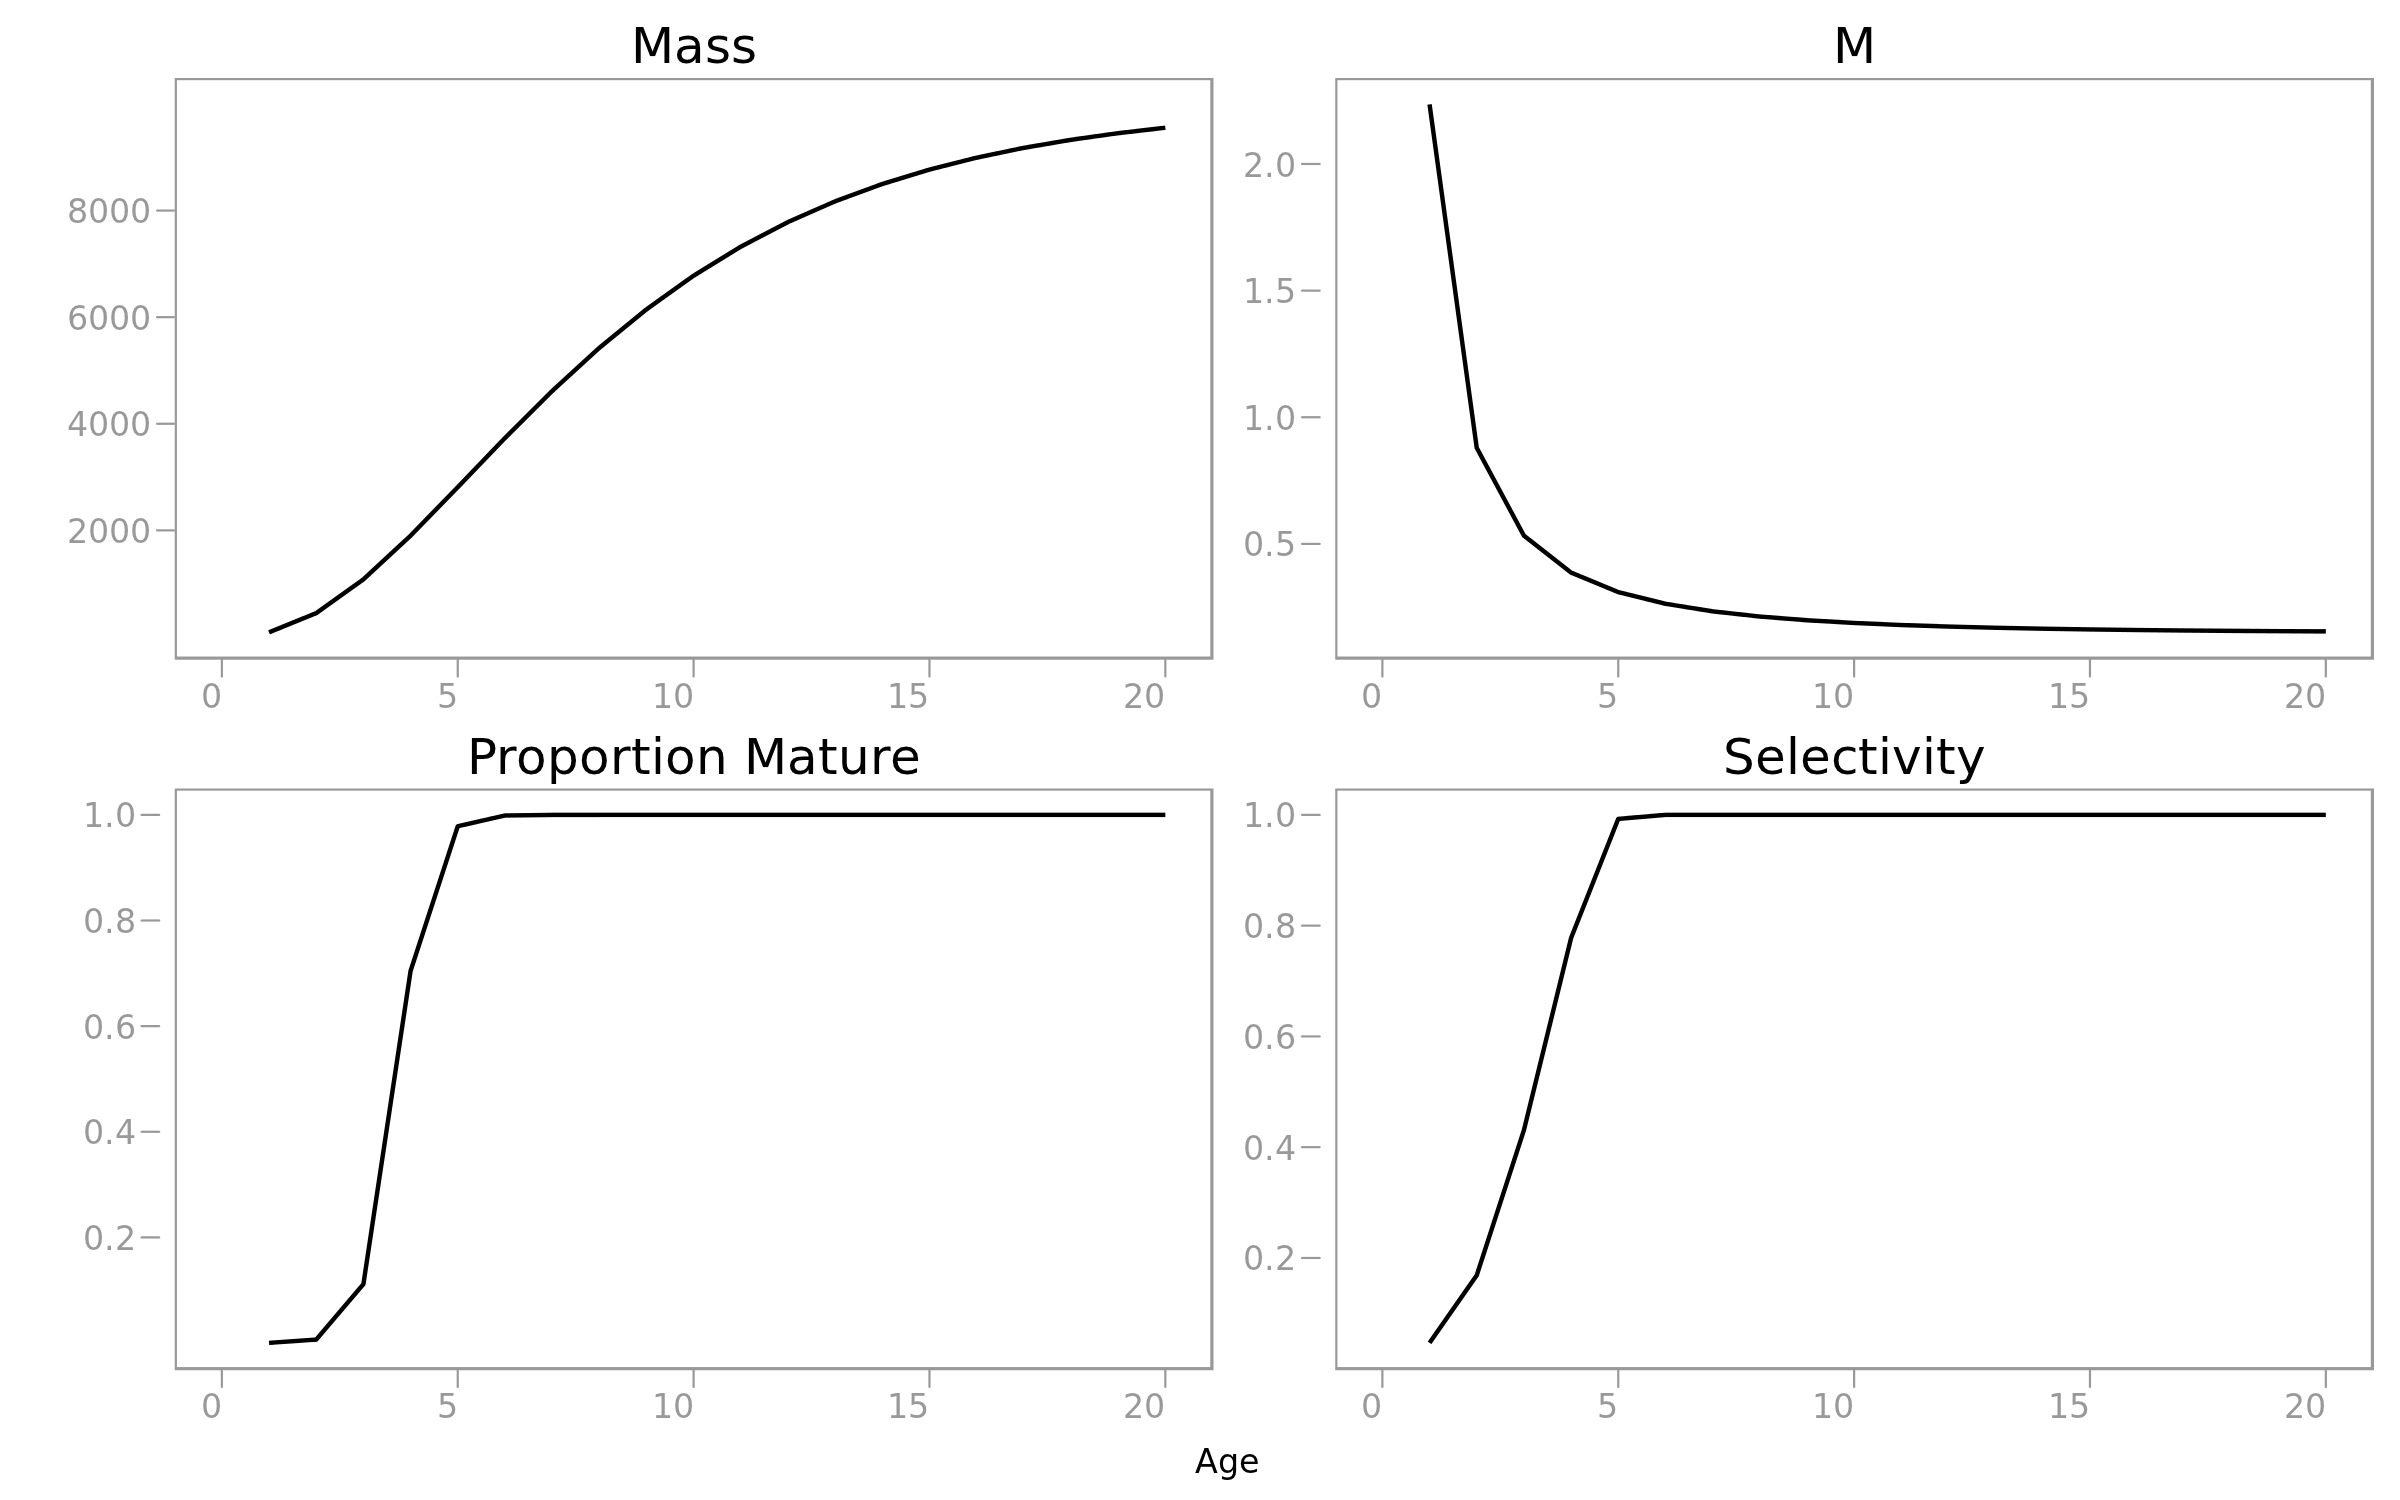
\includegraphics[height=4in, width=4in]{fig1.png}
\end{center}
\caption{\bf{Mass, natural mortality, proportion mature and selection pattern-at-age.}}
\label{fig:stock}
\end{figure}

\begin{figure}[!ht]
\begin{center}
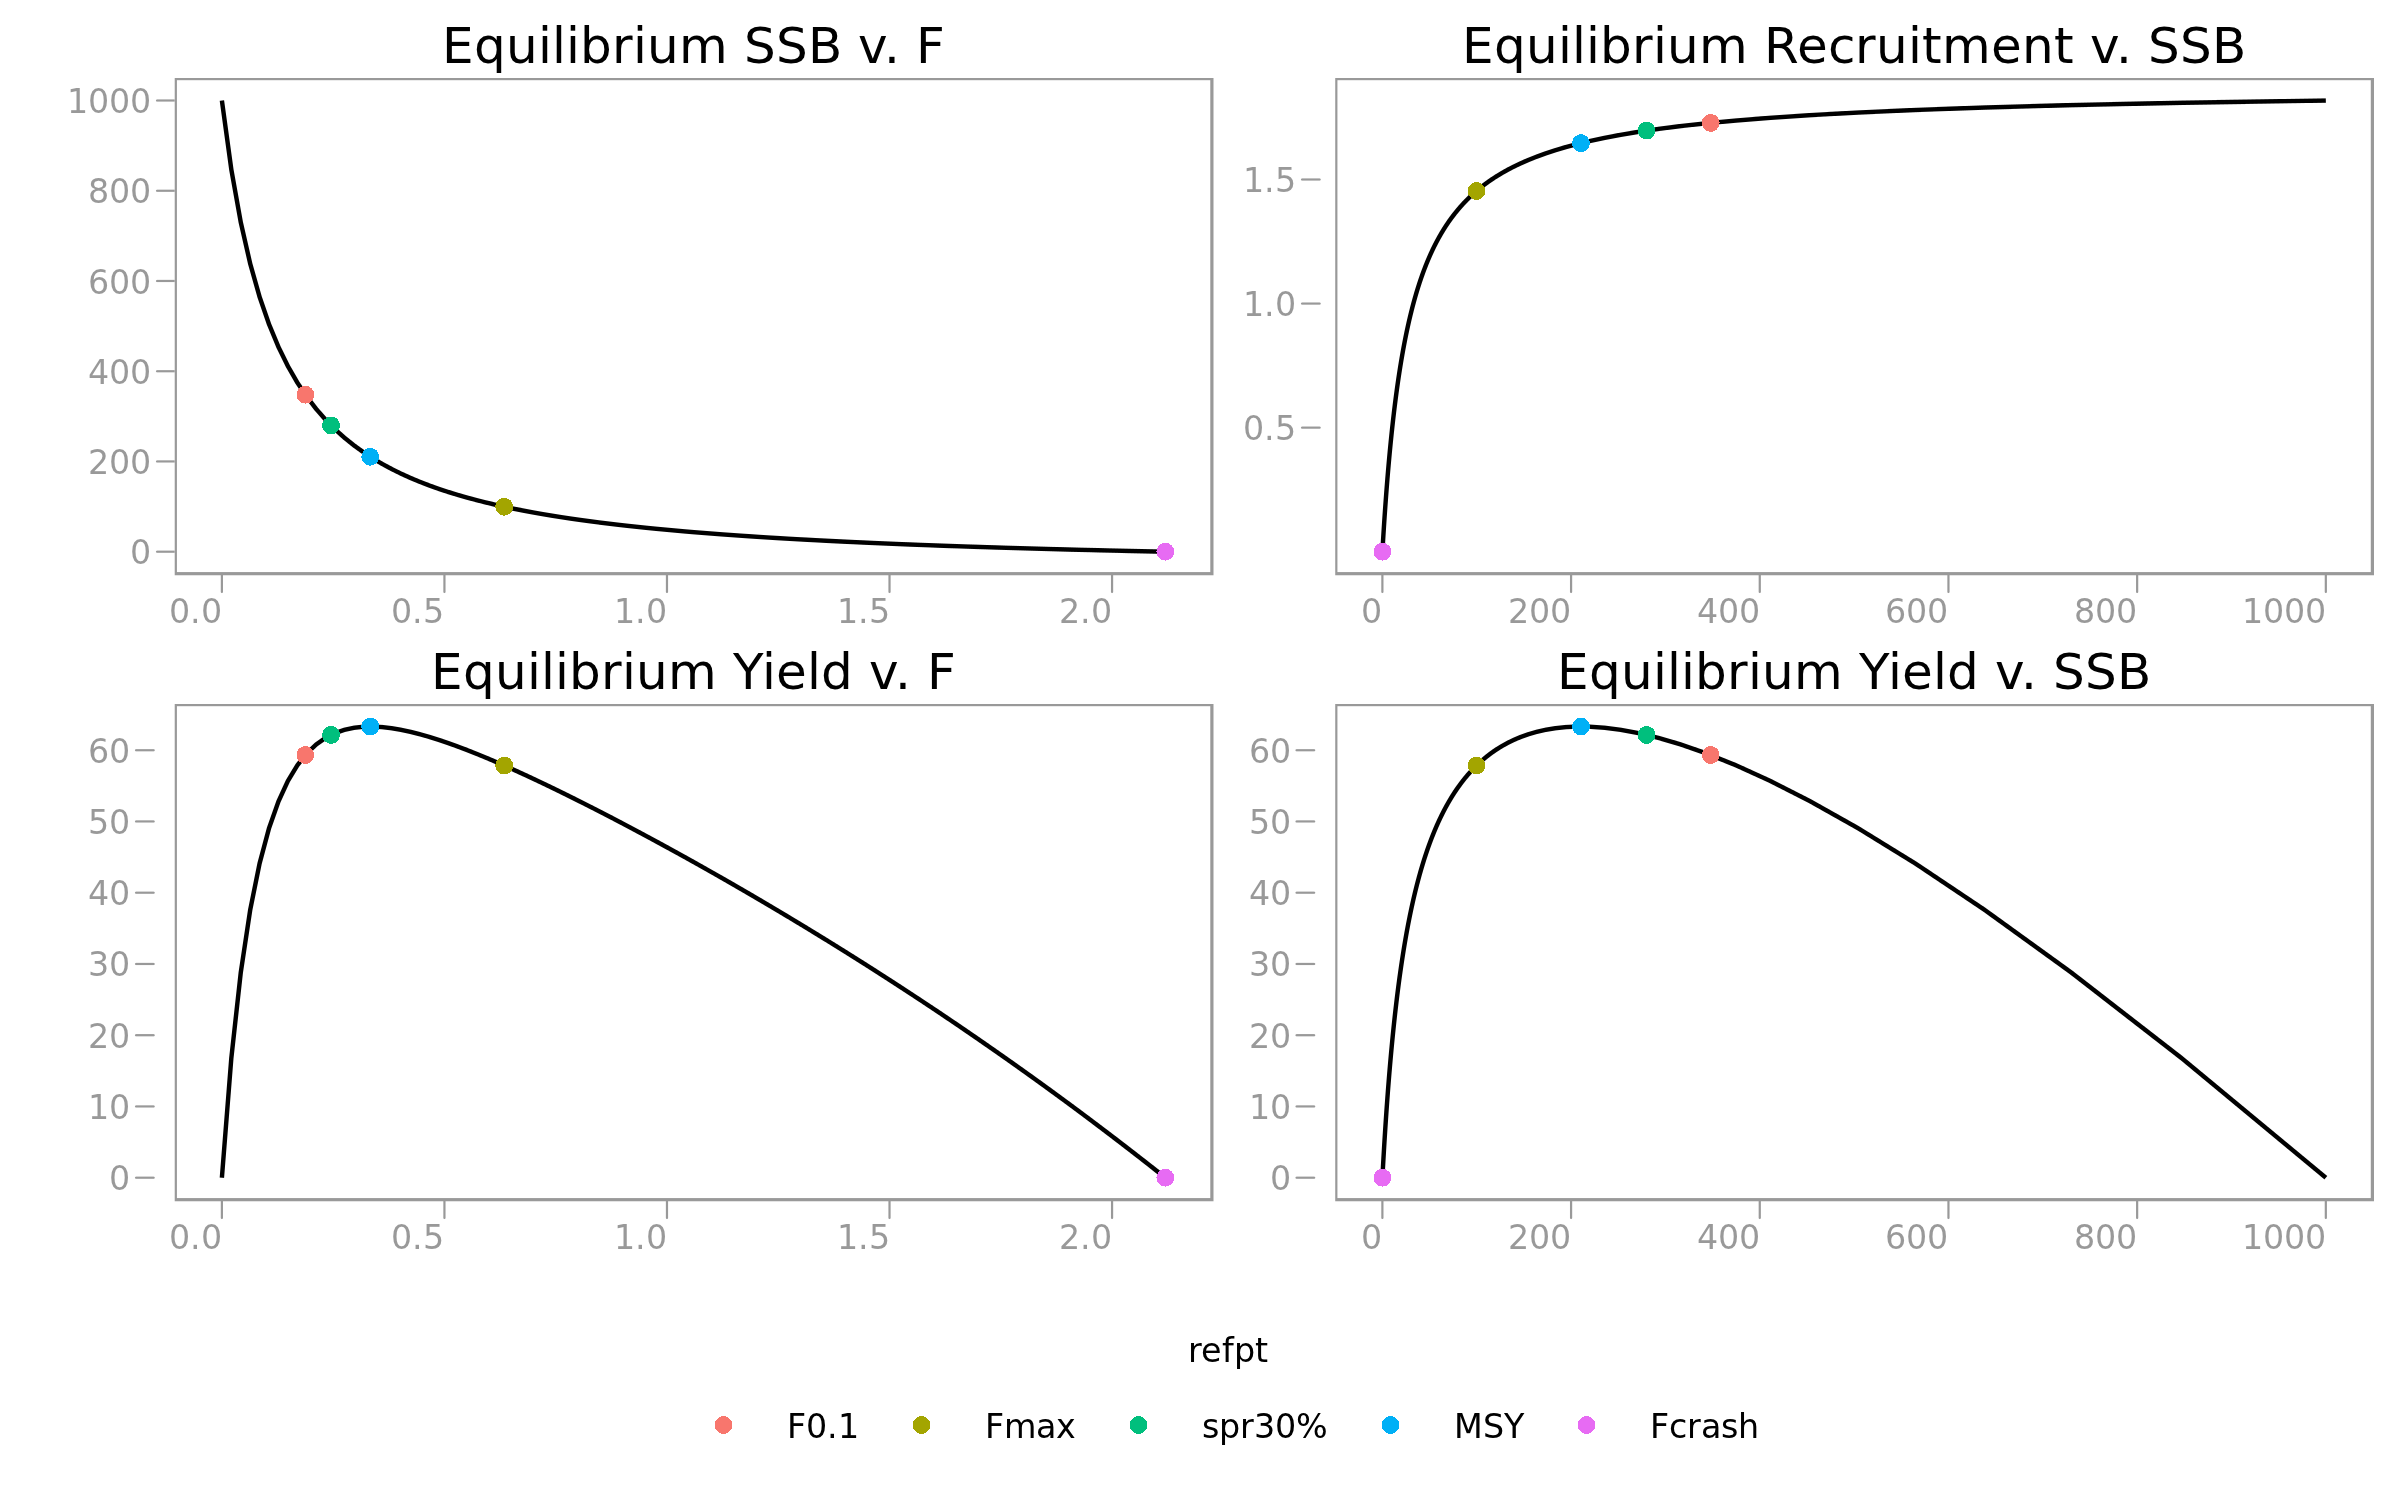
\includegraphics[height=2.1in, width=4in]{fig2.png}
\end{center}
\caption{\bf{Equilibrium (i.e. expected) values of SSB and yield verses fishing mortality and recruitment and yield verses SSB; points correspond to
MSY and MSY proxies ($F_{0.1}$, $F_{Max}$, SPR30\%) and limit ($F_{crash}$) reference points.}}
\label{fig:brp}
\end{figure}

\begin{figure}[!ht]
\begin{center}
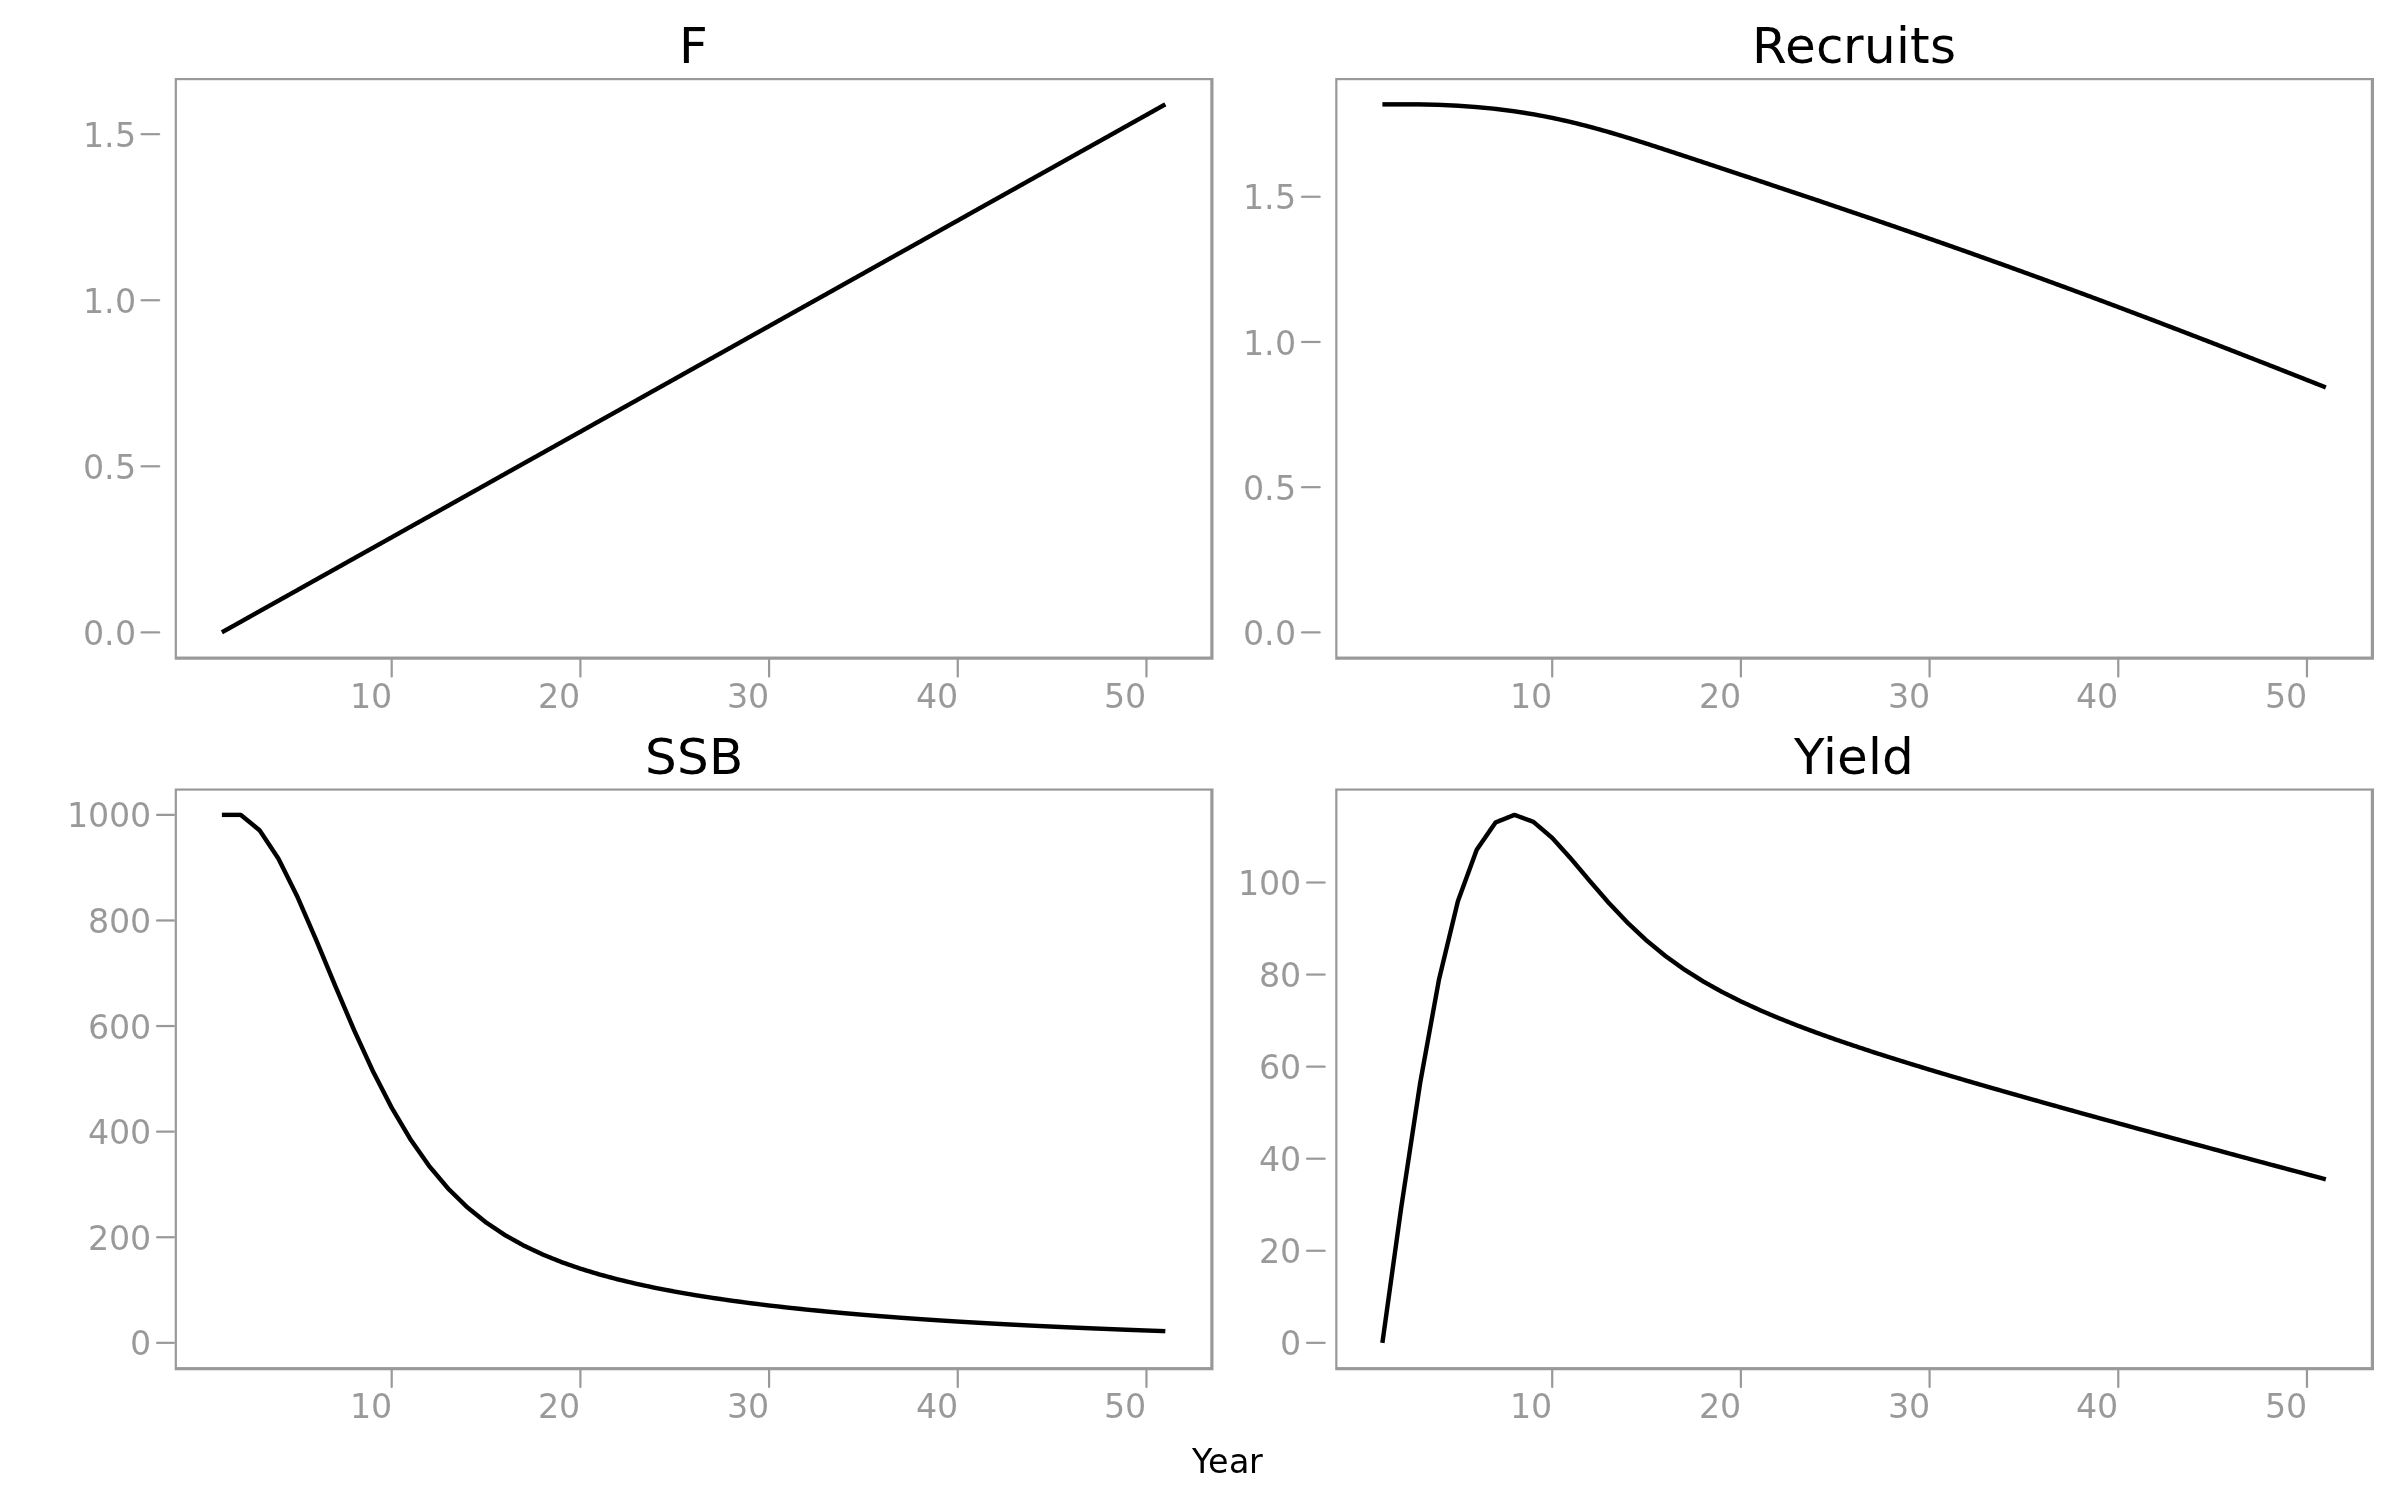
\includegraphics[height=2.1in, width=4in]{fig3.png}
\end{center}
\caption{\bf{Simulated trajectories of recruitment, SSB and yield for a increasing F.}}
\label{fig:kobe}
\end{figure}

\begin{figure}[!ht]
\begin{center}
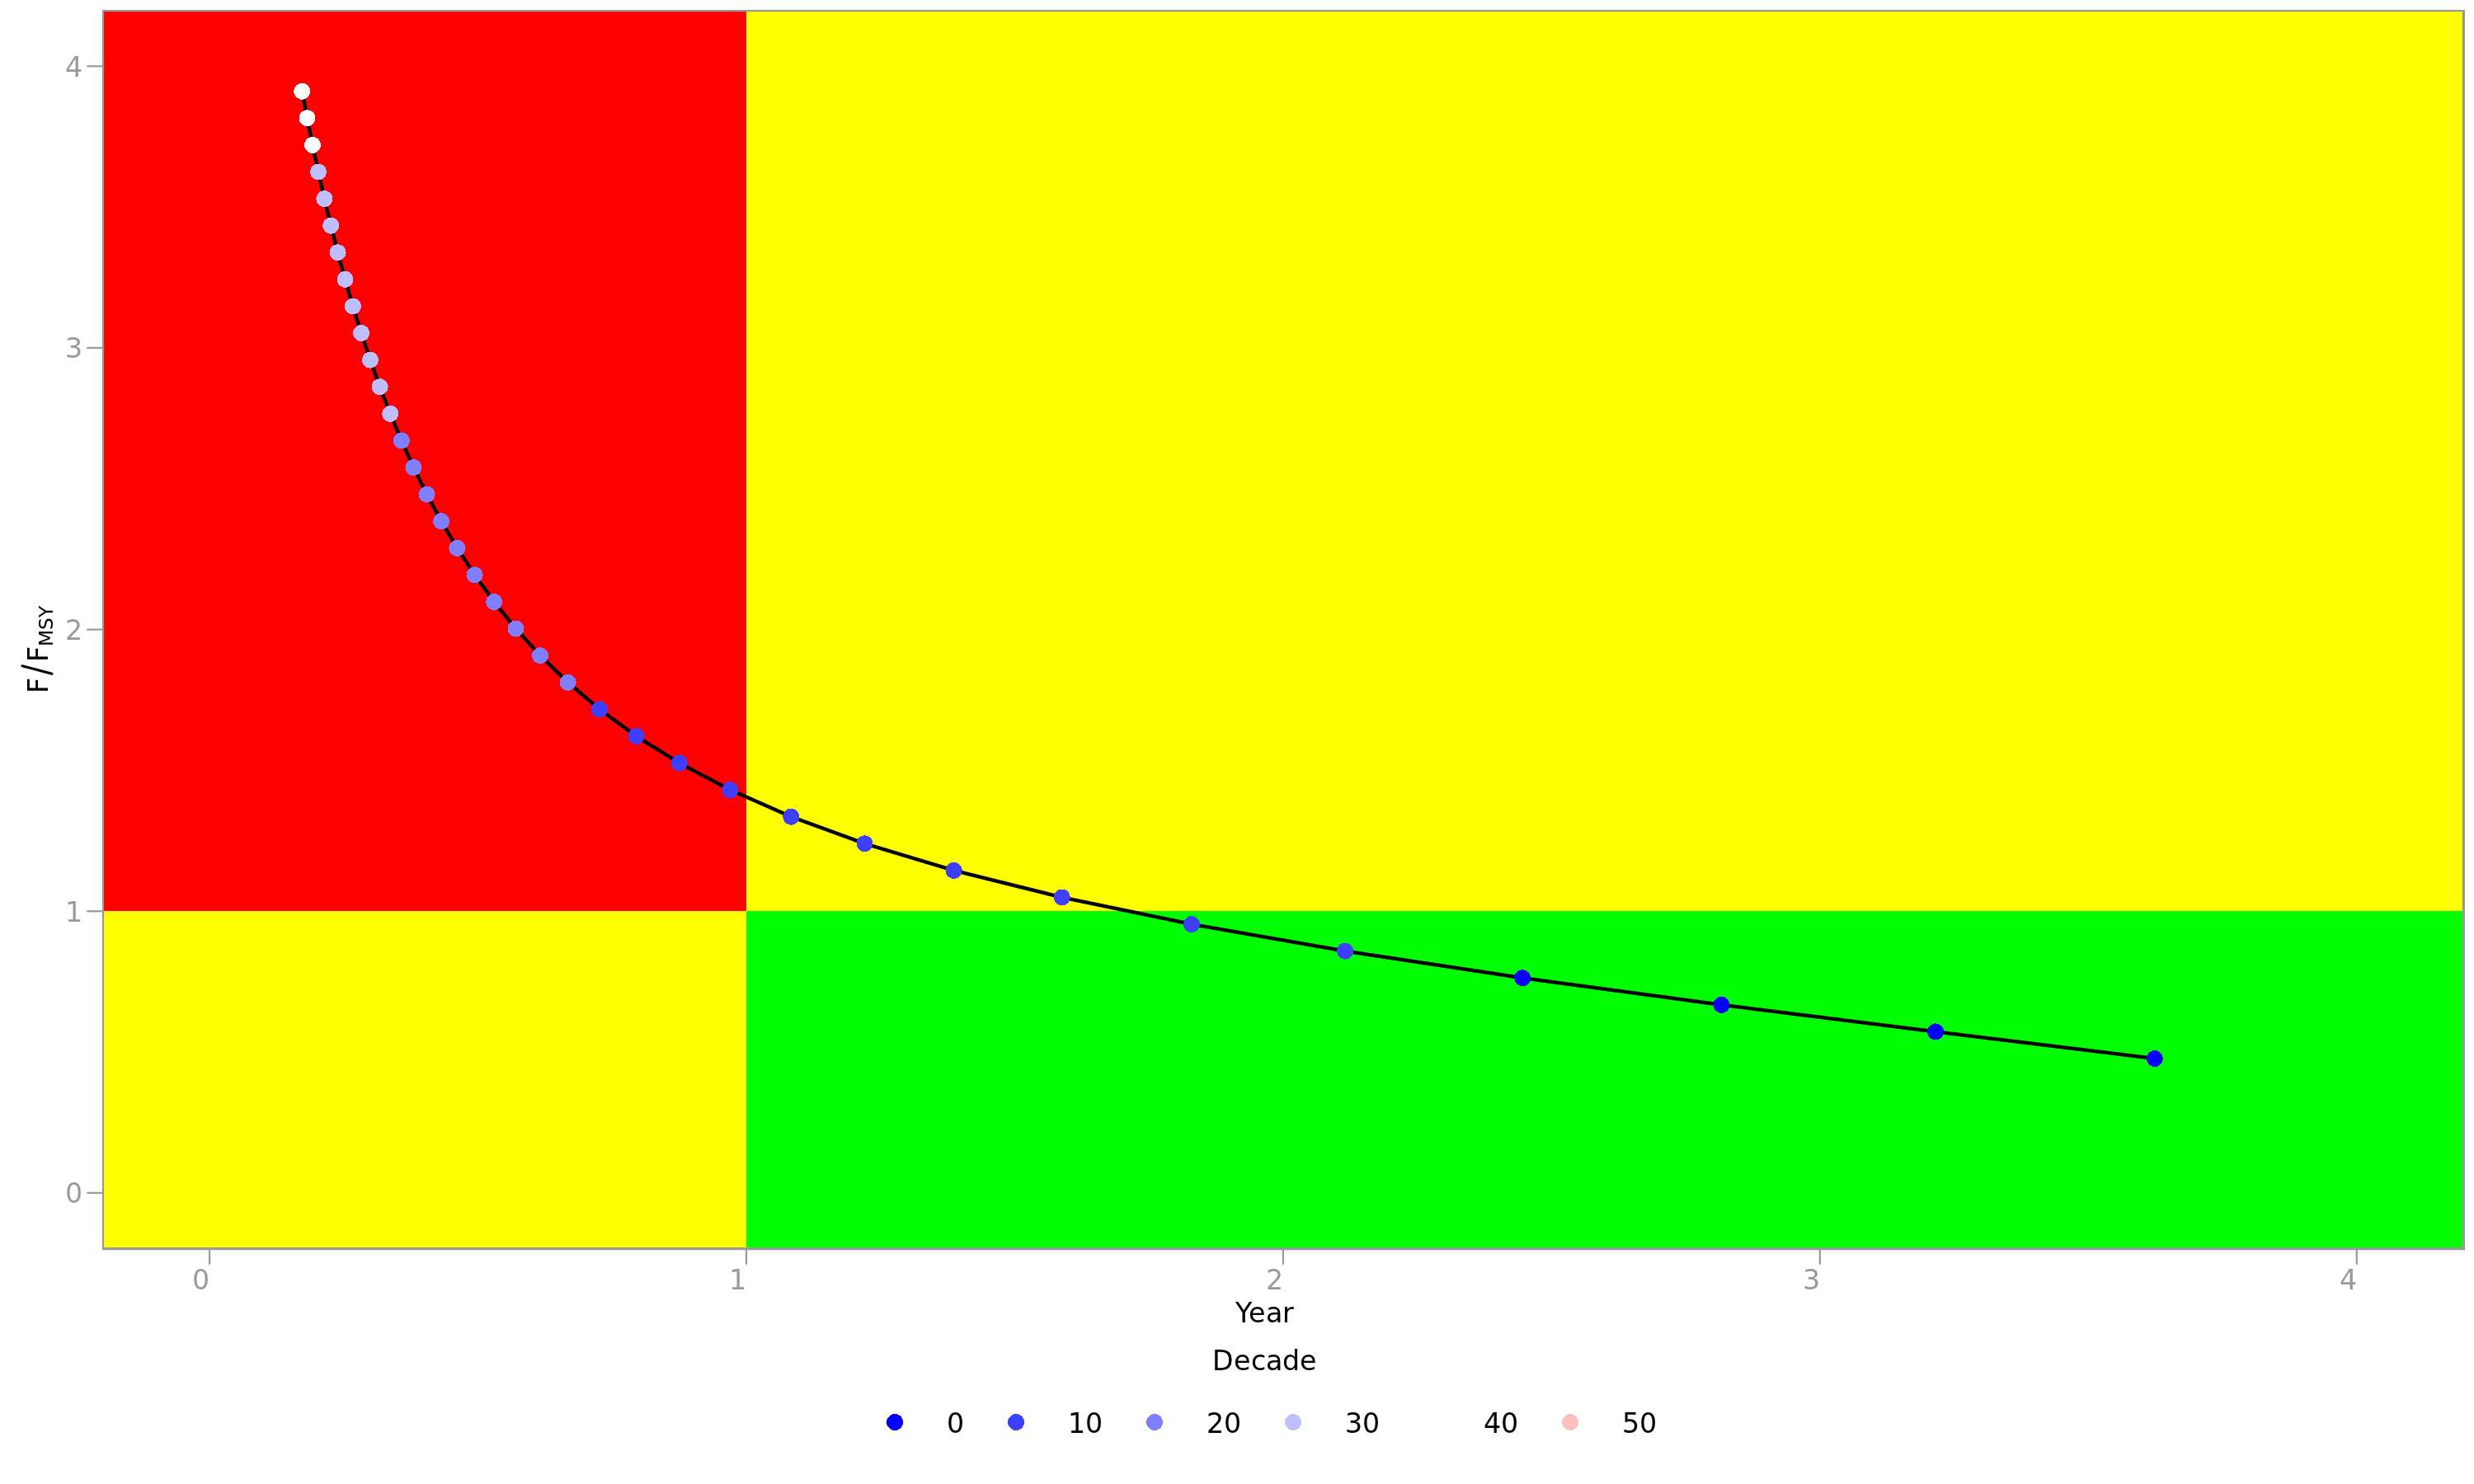
\includegraphics[height=6in, width=6in]{fig4.png}
\end{center}
\caption{\bf{Plots of elasticities of SSB relative to the MSY, $F_{0.1}$ and $F_{crash}$ reference points.}}
\label{fig:elasssb}
\end{figure}

\begin{figure}[!ht]
\begin{center}
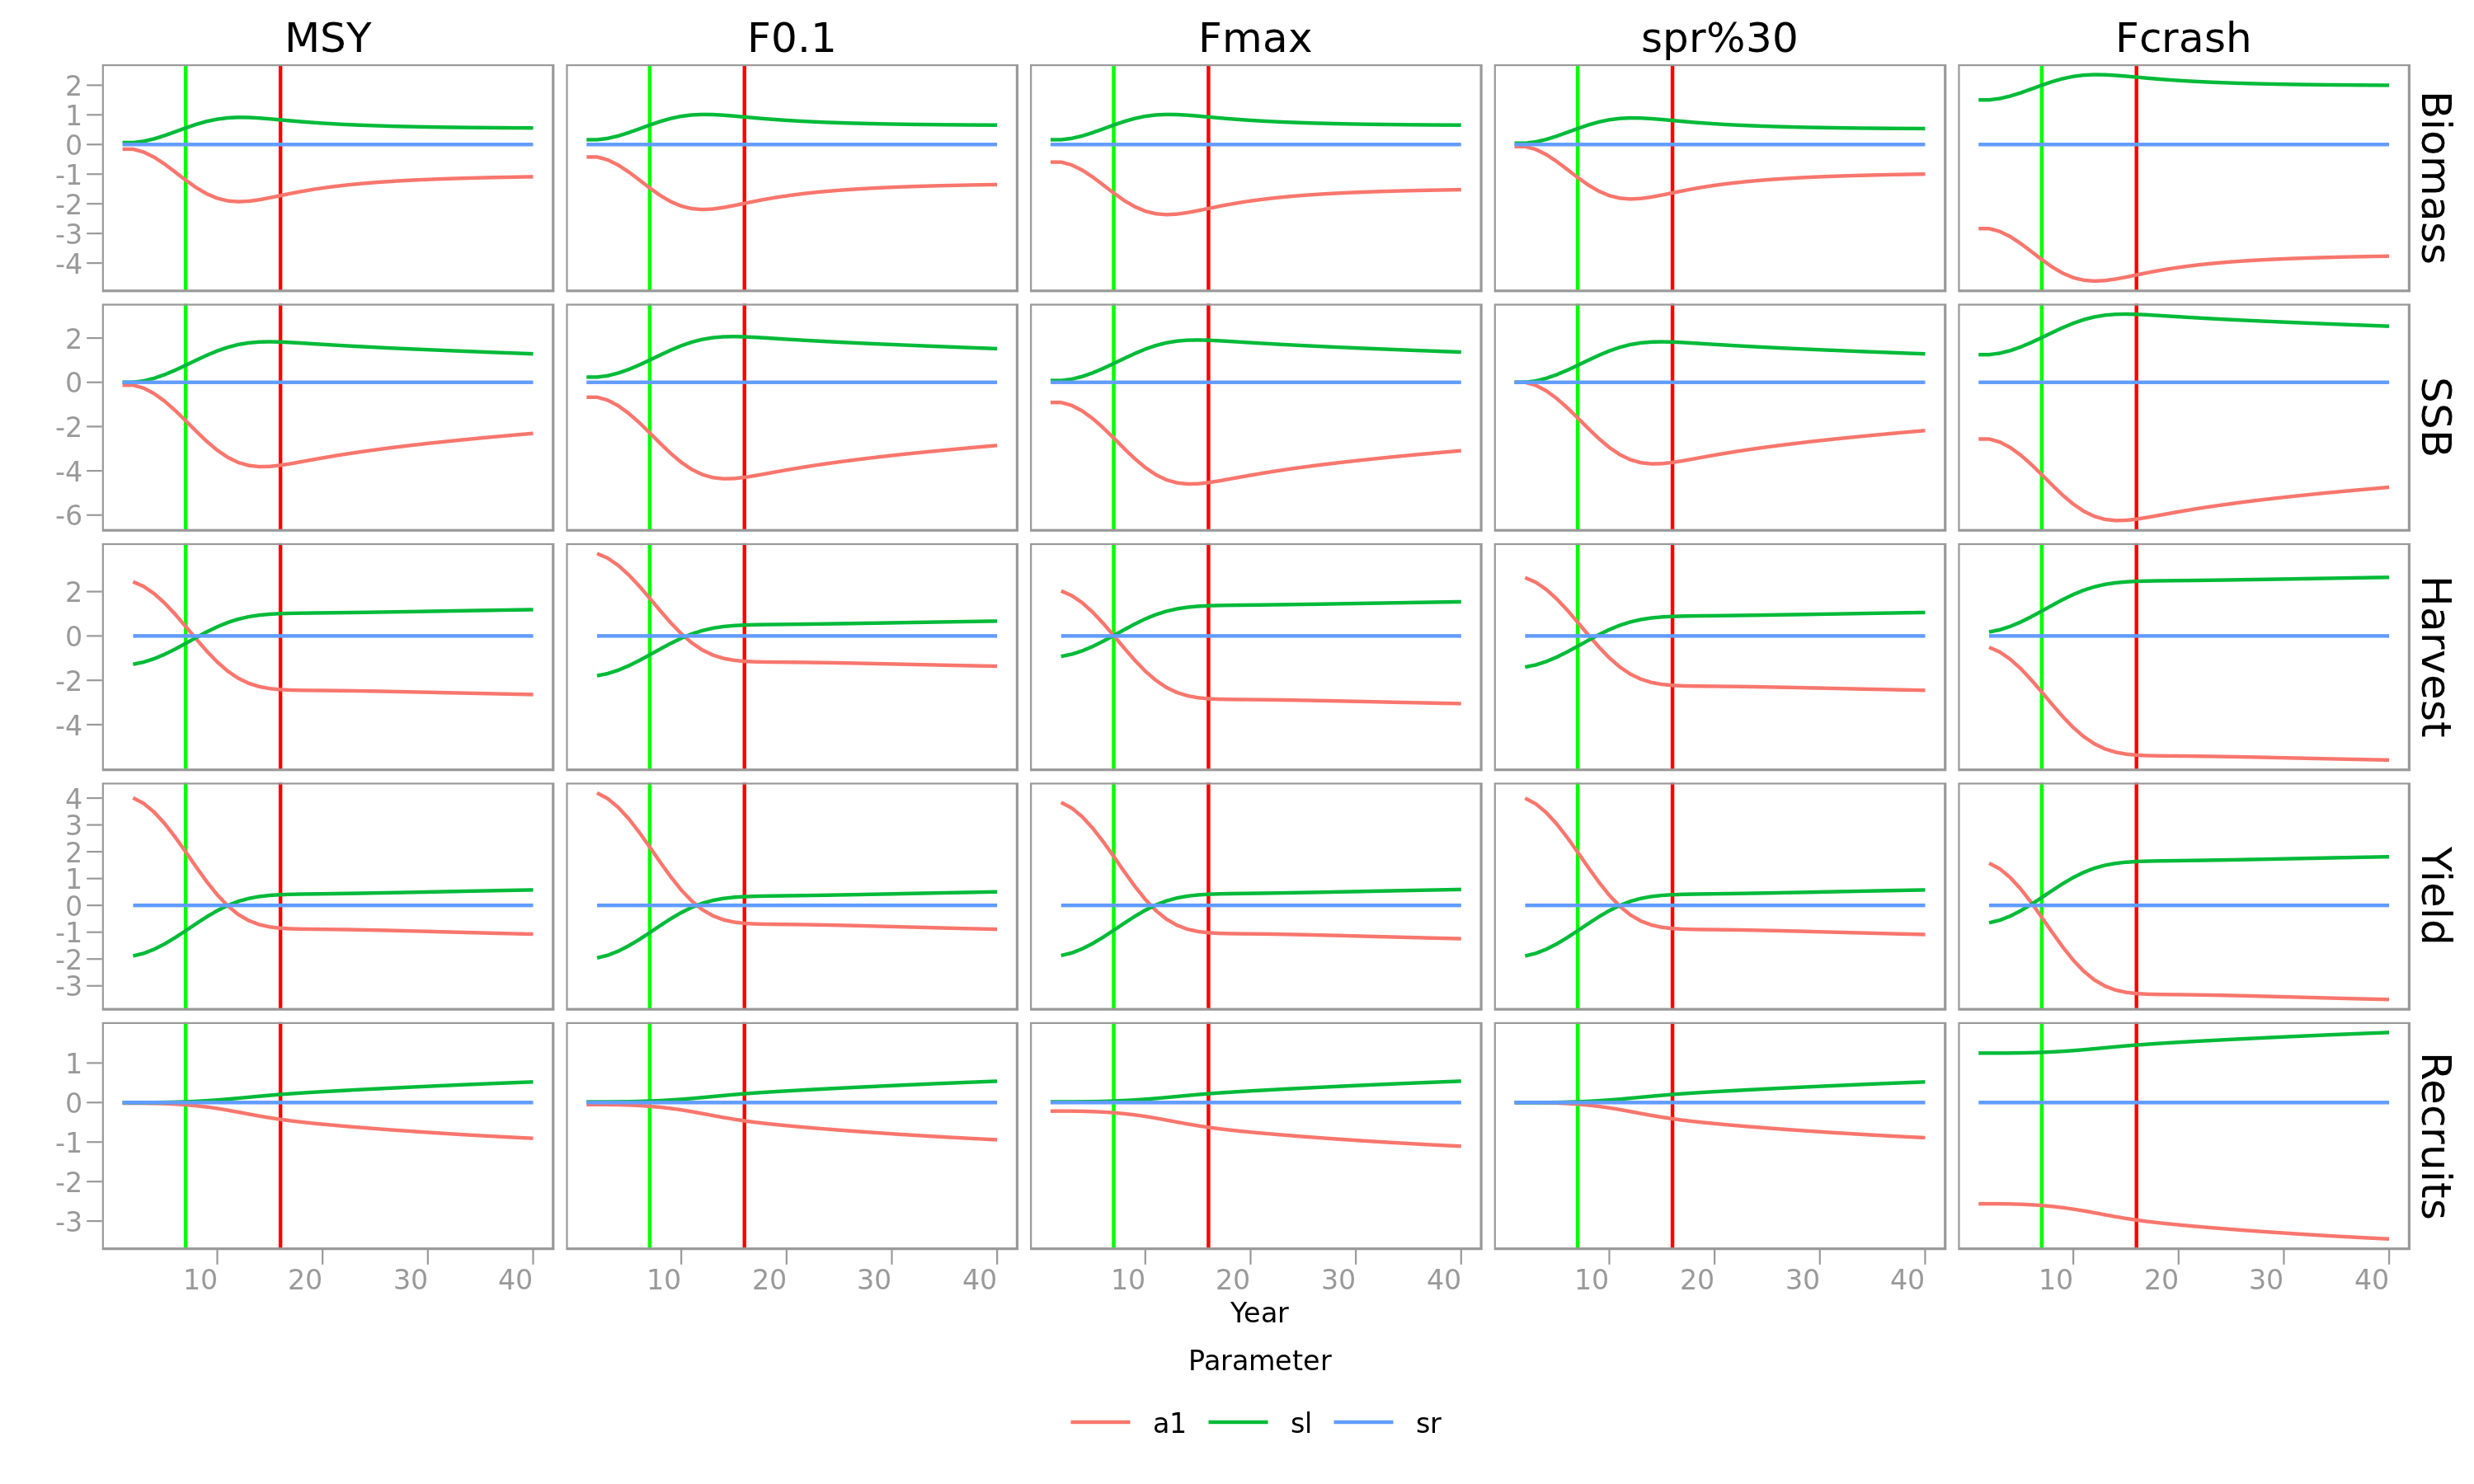
\includegraphics[height=6in, width=6in]{fig5.png}
\end{center}
\caption{\bf{Plots of elasticities of F relative to the MSY, $F_{0.1}$ and $F_{crash}$ reference points.}}
\label{fig:elasf}
\end{figure}


\section*{Tables}
%\begin{table}[!ht]
%\caption{
%\bf{Table title}}
%\begin{tabular}{|c|c|c|}
%table information
%\end{tabular}
%\begin{flushleft}Table caption
%\end{flushleft}
%\label{tab:label}
% \end{table}

\end{document}

